\documentclass[aspectratio=169]{beamer}
%\documentclass[aspectratio=43]{beamer}

\usepackage{graphicx}  % Required for including images
\usepackage{natbib}
\usepackage{booktabs} % Top and bottom rules for tables
\usepackage{amssymb,amsthm,amsmath}
\usepackage{exscale}
\usepackage{natbib}
\usepackage{tikz}
\usepackage{listings}
\usepackage{color}
\usepackage{animate}
\usepackage{bm}
\usepackage{etoolbox}

% Setup TikZ
\usepackage{tikz}
\usetikzlibrary{arrows}
\tikzstyle{block}=[draw opacity=0.7,line width=1.4cm]
% Setup hyperref
\usepackage{hyperref}
\hypersetup{colorlinks=true}
\hypersetup{citecolor=porange}
\hypersetup{urlcolor=porange!80!}
\hypersetup{linkcolor=porange}

\newtheorem{proposition}{Proposition}
\newtheorem{remark}{Remark}
\newtheorem{principle}{Principle}

%% Writing quarters
\newcommand{\wQ}[1]{{\textcolor{white}{Q#1}}}
\newcommand{\bQ}[1]{{Q#1}}

% Uncomment appropriate command to disable/enable hiding
\newcommand{\mypause}{\pause}
%\newcommand{\mypause}{}
\newcommand{\myb}[1]{{\color{blue} {#1}}}

%% Commonly used macros
\newcommand{\eqr}[1]{Eq.\thinspace(#1)}
\newcommand{\pfrac}[2]{\frac{\partial #1}{\partial #2}}
\newcommand{\pfracc}[2]{\frac{\partial^2 #1}{\partial #2^2}}
\newcommand{\pfraca}[1]{\frac{\partial}{\partial #1}}
\newcommand{\pfracb}[2]{\partial #1/\partial #2}
\newcommand{\pfracbb}[2]{\partial^2 #1/\partial #2^2}
\newcommand{\spfrac}[2]{{\partial_{#1}} {#2}}
\newcommand{\mvec}[1]{\mathbf{#1}}
\newcommand{\gvec}[1]{\boldsymbol{#1}}
\newcommand{\script}[1]{\mathpzc{#1}}
\newcommand{\eep}{\mvec{e}_\phi}
\newcommand{\eer}{\mvec{e}_r}
\newcommand{\eez}{\mvec{e}_z}
\newcommand{\iprod}[2]{\langle{#1}\rangle_{#2}}

\DeclareMathAlphabet{\mathpzc}{OT1}{pzc}{m}{it}

%% Autoscaled figures
\newcommand{\incfig}{\centering\includegraphics}
\setkeys{Gin}{width=0.9\linewidth,keepaspectratio}

%Make the items smaller
\newcommand{\cramplist}{
	\setlength{\itemsep}{0in}
	\setlength{\partopsep}{0in}
	\setlength{\topsep}{0in}}
\newcommand{\cramp}{\setlength{\parskip}{.5\parskip}}
\newcommand{\zapspace}{\topsep=0pt\partopsep=0pt\itemsep=0pt\parskip=0pt}

\newcommand{\backupbegin}{
   \newcounter{finalframe}
   \setcounter{finalframe}{\value{framenumber}}
}
\newcommand{\backupend}{
   \setcounter{framenumber}{\value{finalframe}}
}

\usetheme[bullet=circle,% Use circles instead of squares for bullets.
          titleline=true,% Show a line below the frame title.
          ]{Princeton}

\title[{\tt }]{Hyperbolic PDEs and Finite-Volume Methods IV}%
\author[https://ast560.rtfd.io]%
{Ammar H. Hakim ({\tt ammar@princeton.edu}) \inst{1}}%

\institute[PPPL]
{ \inst{1} Princeton Plasma Physics Laboratory, Princeton, NJ %
}

\date[3/23/2021]{Princeton University, Course AST560, Spring 2021}

\begin{document}

\begin{frame}[plain]
  \titlepage
\end{frame}

\begin{frame}{Steps in constructing finite-volume method}
  \begin{align*}
    \pfrac{\mvec{Q}_j}{t} + \frac{\mvec{G}(\mvec{Q}_{j+1/2}^+,\mvec{Q}_{j+1/2}^-) - \mvec{G}(\mvec{Q}_{j-1/2}^+,\mvec{Q}_{j-1/2}^-)}{\Delta x} = 0    
  \end{align*}
  To completely specify a finite-volume scheme we must design
  algorithms for each of the following three steps:
  \begin{itemize}\cramplist
  \item {\bf Step 1}: A {\bf recovery scheme} (possibly with limiters)
    to compute the left/right interface values $\mvec{Q}^{\pm}$ at
    each interface using a set of cell-average values around that
    interface,%
    \mypause%
  \item {\bf Step 2}: A {\bf numerical flux function} that takes the
    left/right values and returns a consistent approximation to the
    physical flux, and%
    \mypause%
  \item {\bf Step 3}: A {\bf time-stepping scheme} to advance the
    solution in time and compute the cell-averages at the next
    time-step.
  \end{itemize}
\end{frame}

\begin{frame}{Essence of the finite-volume method}
  \footnotesize
  \begin{columns}
  
    \begin{column}{0.5\linewidth}
      Instead of computing one edge value we will compute \emph{two}
      values: one the left and one on right of cell-edge. We will next
      define a \emph{numerical flux function}
      \begin{align*}
        \mvec{G} = \mvec{G}(\mvec{Q}^{-}_{j+1/2},\mvec{Q}^{+}_{j+1/2})
      \end{align*}
      with \emph{consistency} condition
      \begin{align*}
        \lim_{\mvec{Q}_{L,R}\rightarrow Q} \mvec{G}(\mvec{Q}_L,\mvec{Q}_R) = \mvec{F}(\mvec{Q})
      \end{align*}
    \end{column}
  
    \begin{column}{0.5\linewidth}
      \begin{figure}    
        \setkeys{Gin}{width=0.7\linewidth,keepaspectratio}
        \incfig{FV-1D-grid.pdf}
      \end{figure}    
    \end{column}
  \end{columns}
  \mypause%
  In terms of the numerical flux function the FV update formula
  becomes
  \begin{align*}
    \pfrac{\mvec{Q}_j}{t} + \frac{\mvec{G}(\mvec{Q}_{j+1/2}^+,\mvec{Q}_{j+1/2}^-) - \mvec{G}(\mvec{Q}_{j-1/2}^+,\mvec{Q}_{j-1/2}^-)}{\Delta x} = 0    
  \end{align*}
\end{frame}

\begin{frame}{Numerical Flux Function}
  \footnotesize%
  The numerical flux function computes a \emph{consistent} flux at the
  cell-edge from the cell averages.
  \begin{align*}
    \lim_{\mvec{Q}_{L,R}\rightarrow Q} \mvec{G}(\mvec{Q}_L,\mvec{Q}_R) = \mvec{F}(\mvec{Q}).
  \end{align*}
  Examples
  \begin{itemize}
  \item \emph{Central Flux} in which we simply average the flux from
    the two states at the interface
    \begin{align*}
      \mvec{G}(\mvec{Q}_L,\mvec{Q}_R) = \frac{1}{2}
      \left( \mvec{F}(\mvec{Q}_L) + \mvec{F}(\mvec{Q}_R) \right) .
    \end{align*}
  \item \emph{Upwind Flux} in which we choose the edge on the
    ``upwind'' side to account for direction of information flow:
    \begin{align*}
      \mvec{G}(\mvec{Q}_L,\mvec{Q}_R) = \mvec{F}(\mvec{Q}_L)
    \end{align*}
    if information is flowing from left-to-right, and
    \begin{align*}
      \mvec{G}(\mvec{Q}_L,\mvec{Q}_R) = \mvec{F}(\mvec{Q}_R)
    \end{align*}
    if information is flowing from right-to-left. Begs the question:
    how to determine which direction information is flowing in?
    Answer: the eigensystem of the hyperbolic equation contains this!
  \end{itemize} 
\end{frame}

\begin{frame}{Numerical Flux Function: Lax flux}
  \small%
  \begin{itemize}
  \item A good choice of the numerical flux function is the
    \emph{local Lax} flux:
    \begin{align*}
      \mvec{G}(\mvec{Q}_L,\mvec{Q}_R) = \frac{1}{2}
      \left( \mvec{F}(\mvec{Q}_L) + \mvec{F}(\mvec{Q}_R) \right)
      - \frac{|\lambda|}{2}( \mvec{Q}_R - \mvec{Q}_L )
    \end{align*}
    where $|\lambda|$ is an estimate of the (absolute) maximum of all
    eigenvalues at the interface.%
    \mypause%
  \item   For advection equation this becomes
    \begin{align*}
      G(f_L,f_R) = \frac{1}{2} a ( f_L + f_R ) - \frac{|a|}{2}( f_R - f_L )
    \end{align*}
    This works for either sign of advection speed $a$, automatically
    giving upwinding.%
    \mypause%
  \item Note $|\lambda|$ is only a local (to the interface)
    \emph{estimate}. You can use a global estimate too: orginal
    formulation by Peter Lax (``Lax fluxes'').
  \end{itemize}

\end{frame}

\begin{frame}{Numerical Flux Function: Systems of equations}
  \small%
  \begin{itemize}
  \item Lax flux is a good ``first'' flux to use. However, notice it
    only takes into account a \emph{single} piece of information:
    maximum eigenvalue.%
    \mypause%
  \item For a \emph{linear system} of equations (Maxwell equation) or
    \emph{locally linearized} nonlinear system we can instead do
    \begin{align*}
      G(Q_R,Q_L) = \frac{1}{2}\big(F(Q_R)+F(Q_L)\big) - \frac{1}{2}(A^+\Delta Q_{R,L} - A^-\Delta Q_{R,L})      
    \end{align*}
    where the \emph{fluctuations} $A^\pm\Delta Q$ are defined as
    \begin{align*}
      A^\pm\Delta Q_{R,L} \equiv \sum_p r^p \lambda^\pm_p (w_R^p-w_L^p) = \sum_p r^p \lambda^\pm_p l^p(Q_R-Q_L).
    \end{align*}
    where $\lambda_p^+ = \max(\lambda_p,0)$ and
    $\lambda_p^- = \min(\lambda_p,0)$.%
    \mypause%
  \item Additional care is needed for nonlinear equations like Euler
    or ideal MHD equations. More on this on Thursday.
  \end{itemize}
\end{frame}  

\begin{frame}{Some notation for use in recovery stencils}
  \footnotesize%
  Example: symmetric recovery across two cells can be written as
  \begin{align*}
    Q_{i+1/2} = \frac{1}{2}(Q_{i+1}+Q_j) = \frac{1}{2}(d_p + d_m) Q_{i+1/2}
  \end{align*}
  Example: central difference scheme for second derivative:
  \begin{align*}
    \frac{\partial^2 Q_i}{\partial x^2}
    = \frac{1}{\Delta x^2} (Q_{i+1} - 2 Q_j + Q_{i-1})
    = \frac{1}{\Delta x^2} (\Delta_p - 2I + \Delta_m) Q_i
  \end{align*}      
  \begin{figure}
    \setkeys{Gin}{width=0.75\linewidth,keepaspectratio}
    \incfig{stencil-ops.png}
    \caption{Basic indexing operators to move from cell to cell, face
      to cell and cell to face.}
  \end{figure}
\end{frame}

\begin{frame}{Recovery scheme: four-cell stencil, centered scheme}
  \footnotesize%
  \begin{figure}
    \setkeys{Gin}{width=0.35\linewidth,keepaspectratio}
    \incfig{4c-stencil.png}
  \end{figure}  
  \begin{itemize}
  \item To construct a four-cell symmetric stencil recovery across an
    interface we will use a four-cell stencil:
    $\{d_{2m}, d_m, d_p, d_{2p} \}$%
    \mypause%
  \item Setup a local coordinate system with $x=0$ at the interface
    and assume a polynomial recovery
    \begin{align*}
      p(x) = p_0 + p_1 x + p_2 x^2 + p_3 x^3
    \end{align*}
    \mypause%
  \item Match the cell-averages of $p(x)$ in each of the cells
    $\{d_{2m}, d_m, d_p, d_{2p} \}$ to get a system of linear
    equations. Solve this system to determine $p_0, p_1, p_2, p_3$.
  \end{itemize}
\end{frame}

\begin{frame}{Recovery scheme: four-cell stencil, centered scheme}
  Solving the system of four equations for the four coefficients
  $p_i$, $i=0,\ldots,3$ yields:
  \begin{align*}
    p_0 &=  \frac{1}{12}(-d_{2m} + 7 d_m + 7 d_p - d_{2p}) Q \\
    p_1 &=  \frac{1}{12\Delta x}(d_{2m} - 15 d_m + 15 d_p - d_{2p}) Q \\
    p_2 &=  \frac{1}{4 \Delta x^2}(d_{2m} - d_m - d_p + d_{2p}) Q \\
    p_4 &=  \frac{1}{6 \Delta x^3}(d_{2m} - 3d_m + 3 d_p - d_{2p}) Q.
  \end{align*}
  \begin{itemize}
  \item Notice: stencils of the even coefficients are \emph{symmetric}
    and the odd coefficients are \emph{anti-symmetric}.%
    \mypause%
  \item To compute the interface value we do not really need all of
    these coefficients but only need to evaluate the recovery
    polynomial at $x=0$, i.e we only need $p(0) = p_0$
  \end{itemize}
\end{frame}

\begin{frame}{Recovery scheme: four-cell stencil, centered scheme}
  \small%
  To compute the interface value we do not really need all of these
  coefficients but only need to evaluate the recovery polynomial at
  $x=0$, i.e we only need $p(0) = p_0$. Hence, the interface value can
  be computed from
  \begin{align*}
    Q^+ = Q^- = \frac{1}{12}(-d_{2m} + 7 d_m + 7 d_p - d_{2p}) Q.
  \end{align*}
  Note that due the symmetric nature of the stencil we have only a
  \emph{single} value at the interface. This means that the numerical
  flux function at an interface is simply
  \begin{align*}
    G(Q,Q) = F(Q)
  \end{align*}
  from consistency requirements.%
  \mypause%
  This completes the spatial finite-volume discretization! The scheme
  one gets from this is very accurate (even ``structure preserving''
  for Maxwell equations), though not very robust in presence of sharp
  gradients. (No Free Lunch)
\end{frame}

\begin{frame}{How accurate is any given scheme?}
  To fix ideas consider we wish to solve the advection equation
  \begin{align*}
    \pfrac{f}{t} + \pfrac{f}{x} = 0
  \end{align*}
  Using the four-cell symmetric recovery scheme to compute interface
  values in the FV update formula we get the semi-discrete scheme
  \emph{five-cell stencil} update formula:
  \begin{align*}
    \pfrac{f_j}{t}
    = -\frac{1}{\Delta x}\int_{x_{j-1/2}}^{x_{j+1//2}}
    \pfrac{f}{x} \thinspace dx
    =
    -\frac{1}{12 \Delta x} (f_{j-2} - 8f_{j-1} + 8 f_{j+1} - f_{j+2})
  \end{align*}
  How accurate is this scheme, or what is its order of convergence?
\end{frame}

\begin{frame}{How accurate is any given scheme? Use Taylor series}
  \footnotesize%
  \begin{itemize}\cramplist
  \item Take a Taylor series polynomial around the cell center of cell
    $I_j = [-\Delta x/2, \Delta x/2]$ locally at $x=0$
    \begin{align*}
      T(x) = \sum_{n=0} \frac{T_n}{n!} x^n.
    \end{align*}
    \mypause%
  \item Compute the cell average of this polynomial in each of the
    stencil cells $\{\Delta_{2m}, \Delta_m, \Delta_p, \Delta_{2p} \}$
    \mypause%
  \item Substitute these averages in the update formula to compute the
    mean value of the flux gradient in the cell
    $I_j = [-\Delta x/2, \Delta x/2]$
    \begin{align*}
      \frac{1}{12 \Delta x} (\Delta_{2m} - 8\Delta_m + 8 \Delta_p -
      \Delta_{2p}) T
      =
      T_1 + \frac{\Delta x^2}{24} T_3  - \frac{21 \Delta x^4}{640} T_5 + \ldots
    \end{align*}
    \mypause%
  \item Subtract the exact cell average of the gradient of the Taylor
    polynomial in cell $I_j = [-\Delta x/2, \Delta x/2]$, i.e.
    \begin{align*}
      \frac{1}{\Delta x}\int_{-\Delta x/2}^{\Delta x/2} \pfrac{T}{x} \thinspace dx
      =
      T_1 + \frac{\Delta x^2}{24} T_3  + \frac{\Delta x^4}{1920} T_5 + \ldots
    \end{align*}
    from the stencil computed value. The remainder term is the error
    of the scheme.
  \end{itemize}  
\end{frame}

\begin{frame}{Symmetric four-cell recovery scheme is fourth-order
    accurate}
  The above procedure (needs use of a compute algebra system to
  simplify the computations) shows that the symmetric four-cell
  recovery scheme has error that goes like
  \begin{align*}
      \frac{\Delta x^4}{30} T_5 + O(\Delta x^6)
  \end{align*}
  showing the scheme converges with \emph{fourth-order} accuracy
  $O(\Delta x^4)$ for linear advection equation. (Reducing $\Delta x$
  by 2 reduces error by a factor of $16$).

\end{frame}

\begin{frame}{Accuracy is not everything: dispersion and diffusion}
  \footnotesize
  \begin{itemize}
  \item High-order symmetric schemes like the one we derived are very
    accurate (even ``structure preserving'' for some problems) but not
    robust.
    \mypause%
  \item Two other properties of the scheme are important to
    understand: \emph{dispersion} and \emph{diffusion}. For this we
    wil derive a \emph{numerical dispersion relation} analogous to
    dispersion relation we derived for linearized systems.
    \mypause%
  \item Consider a single mode $f(x) = e^{ik x}$ where $k$ is the
    wavenumber. Compute the cell-average of the mode on each of the
    cells in the stencil, plug into the stencil formula to derive the
    \emph{numerical dispersion relation}
    \begin{align*}
      i\overline{k} = \sum_{m=-N}^{M} c_m e^{i k m \Delta x}
    \end{align*}
    where we have written the stencil in the generic form
    \begin{align*}
      \frac{1}{\Delta x}\sum_{m = -N}^{M} c_m f_{j+m}
    \end{align*}

  \end{itemize}
\end{frame}

\begin{frame}{Symmetric four-cell recovery scheme has no diffusion!}
  \small
  \begin{columns}
    
    \begin{column}{0.6\linewidth}
      \begin{itemize}
      \item Note that the numerical dispersion relation will in
        general give a \emph{complex} effective wavenumber
        $\overline{k}$.
      \item The dispersion relation for a hyperbolic equation is
        $\omega = \lambda k$. Hence, the \emph{real part} of
        $\overline{k}$ represents dispersion and \emph{imaginary part}
        of $\overline{k}$ represents diffusion/growth. Obviously, we
        want imaginary part to be \emph{negative} to avoid solution
        blow-up!
      \item The four-cell symmetric stencil has \emph{no imaginary
          part} of $\overline{k}$. This related to the fact that it is
        \emph{symmetric} (anti-symmetric stencil coefficients). This
        is not necessarily a good thing!
      \end{itemize}
    \end{column}
  
    \begin{column}{0.4\linewidth}
      \begin{figure}
        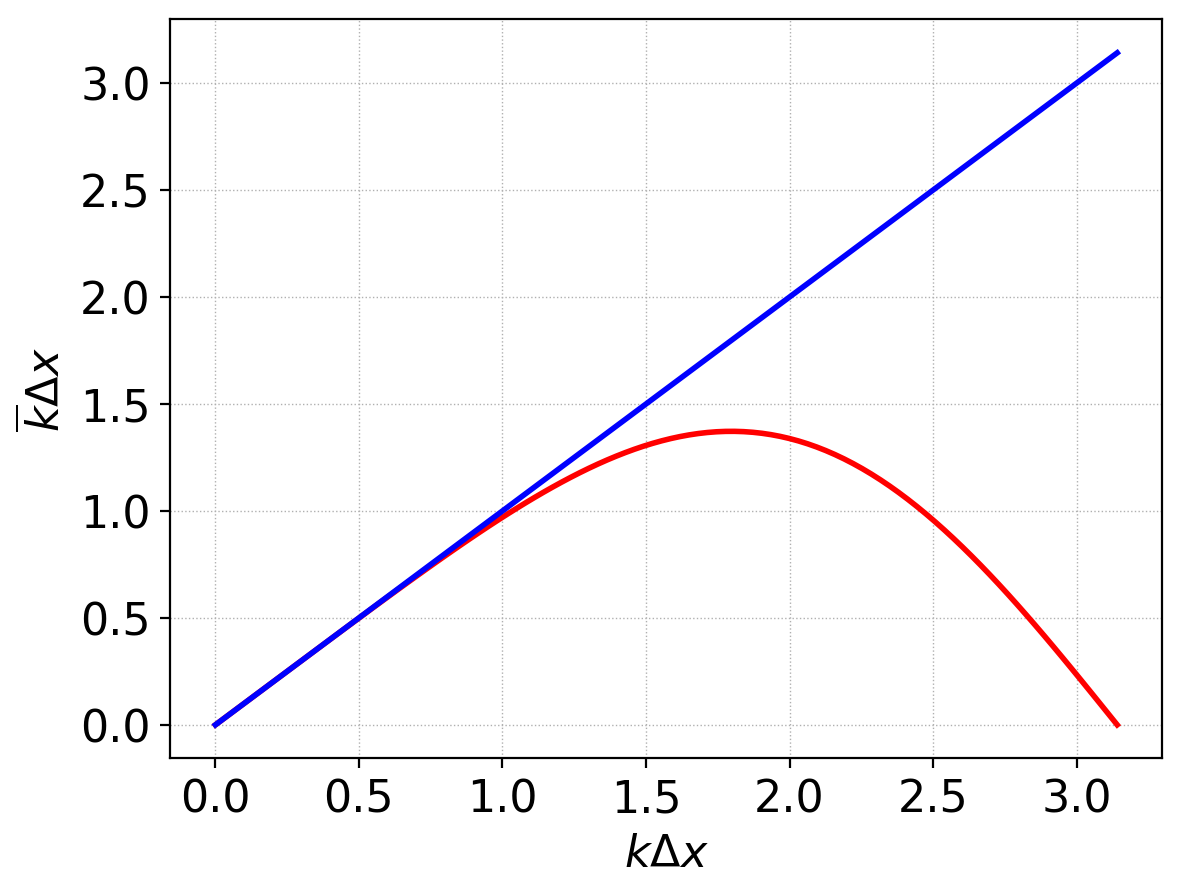
\includegraphics[width=\linewidth]{5p-kbar.png}
        \caption{Real-part of numerical dispersion relation for
          four-cell recovery scheme. Notice the strong dispersion for
          higher-$k$ modes}
      \end{figure}
    \end{column}
  \end{columns}

\end{frame}

\begin{frame}{Closer look at numerical dispersion relation}
  The numerical dispersion relation determines the wave-vector that
  the \emph{time-propagator} of the scheme sees. Consider:
  \begin{align*}
    i\overline{k} = i\overline{k}(k) =  \sum_{m=-N}^{M} c_m e^{i k m \Delta x}
  \end{align*}
  If we are solving a linear advection equation with a single mode
  solution like $e^{-i \omega_k t} e^{i k x}$, where
  $\omega_k = \lambda k$ then the effective mode in the discrete
  scheme will be
  \begin{align*}
    \overline{\omega}_k = \lambda \overline{k}(k).
  \end{align*}
  Hence, the numerical scheme adds \emph{numerical dispersion} to
  propagating waves as now the phase- and group-velocity are no longer
  constant.

\end{frame}  


\begin{frame}{Godunov's Theorem}
  \small%
  \begin{itemize}
  \item A very important theorem proved by Godunov is that there is {
      \bf no} \emph{linear scheme} that is ``monotonicity preserving''
    (no new maxima/minima created) and {\bf higher than first-order
      accurate}!  \mypause%
  \item Consider a general scheme for advection equation
    \begin{align*}
      f_j^{n+1} = \sum_k c_k f_{j+k}^n.
    \end{align*}
    The discrete slope then is
    \begin{align*}
      f_{j+1}^{n+1} - f_j^{n+1} = \sum_k c_k \left( f_{j+k+1}^n - f_{j+k}^n \right).
    \end{align*}
    Assume that all $f_{j+1}^n - f_j^n > 0$. To maintain monotonicity
    at next time-step hence one must have all $c_k \ge 0$.
  \end{itemize}
\end{frame}

\begin{frame}{Godunov's Theorem}
  \small%
  \begin{itemize}
  \item First order upwind scheme:
    \begin{align*}
      f_j^{n+1} = f_j^n -\frac{\Delta t}{\Delta x}(f_j^n - f_{j-1}^n)
    \end{align*}
    this satisfies monotonicity as long as
    ${\Delta t}/{\Delta x} \le 1$.%
    \mypause%
  \item Second order symmetric scheme
    \begin{align*}
      f_j^{n+1} = f_j^n -\frac{\Delta t}{2 \Delta x}(f_{j+1}^n - f_{j-1}^n)
    \end{align*}
    clearly this does not satisfy the condition of monotonicity.
    \mypause%
  \item In general condition on Taylor series to ensure atleast
    second-order accuracy shows that at least \emph{one} of the $c_k$s
    must be negative. Hence, by contradiction, \emph{no such scheme
      exists}!
  \end{itemize}
\end{frame}

\begin{frame}{Godunov's Theorem: Unfortunate Consequences and Workarounds}
  \small%
  \begin{itemize}
  \item Godunov's Theorem is highly distressing: accurate
    discretization seems to preclude a scheme free from monotonicity
    violations
    \mypause%
  \item One way around is to start with a linear scheme that is very
    accurate and then add some local diffusion to it to control the
    monotonicity.%
    \mypause%
  \item However, Godunov's theorem shows that this ``diffusion'' must
    be dependent on the local solution itself and can't be fixed
    \emph{a priori}. This means a {\bf monotonicity preserving scheme
      must be nonlinear}, even for linear hyperbolic equations.%
    \mypause%
  \item Leads to the concept of \emph{nonlinear limiters} that control
    the monotonicity violations (adding diffusion to high-$k$ modes).
    No free lunch: limiters must diffuse high-$k$ modes but this will
    inevitably lead to issues like inability to capture, for example,
    high-$k$ turbulence spectra correctly without huge grids.
  \item Major research project: interaction of shocks, boundary layers
    and turbulence in high-Reynolds number flows.
  \end{itemize}
\end{frame}
  
\end{document}


\begin{frame}{}
\end{frame}

\begin{columns}
  
  \begin{column}{0.6\linewidth}
  \end{column}
  
  \begin{column}{0.4\linewidth}
    \includegraphics[width=\linewidth]{fig/Kinsey_2011_Pfus_vs_T.pdf}
  \end{column}
\end{columns}

% ----------------------------------------------------------------
